\section{Data Visualization}
Data visualization means drawing graphic displays to show data and is generally the first step of machine learning. It gives an  intuitive understanding of data structure,  helps to see trends, clusters, patterns which we don't see in raw data.

\subsection{Plot Types}
\textbf{Components:} X \& Y-Axis Labels, Title, Scale (linear vs logarithmic), Dimensionallity.

\subsubsection{Line Plots}
The line connects several distinct data points, presenting them as one continuous evolution. The result is a simple, straightforward way to visualize changes in one value relative to another.

\subsubsection{Bar Chart}
Often used for categorical data where binning/counting  is done based on each category. 

\subsubsection{Histogramm}
A histogram represents the empirical distribution of a variable by automatically creating bins (interval) along the range of values and by showing vertical bars to indicate the number of observation in each bin.\\

\begin{minipage}{0,5\linewidth}
    \subsubsection{Descriptive Statistics}
    Image to the right.
    \subsubsection{Scatter Plot}
    To understand the relationship between two continuous variables a scatterplot can be used.
\end{minipage}
\begin{minipage}{0,5\linewidth}
    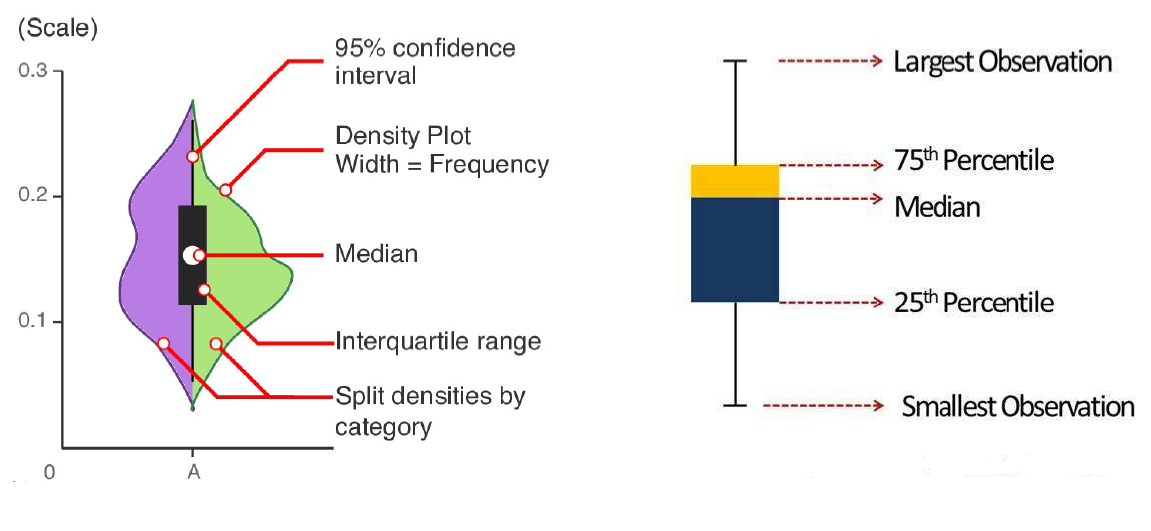
\includegraphics{descriptive_statistics}
\end{minipage}

